\documentclass{ntmanuscript}
\usepackage[acronym,toc]{glossaries}
\newacronym{MIT}{MIT}{the Massachusettes Institute of Technology}
\newacronym{UW}{UW}{University of Wisconsin}
\newacronym{US}{US}{United States}
\newacronym{IAEA}{IAEA}{International Atomic Energy Agency}
\newacronym{SNF}{SNF}{spent nuclear fuel}
\newacronym{HLW}{HLW}{high level waste}
\newacronym{FEHM}{FEHM}{Finite Element Heat and Mass Transfer}
\newacronym{DOE}{DOE}{Department of Energy}
\newacronym{GENIUSv1}{GENIUS}{Global Evaluation of Nuclear Infrastructure 
Utilization Scenarios, Version 1}
\newacronym{GENIUSv2}{GENIUS}{Global Evaluation of Nuclear Infrastructure Utilization Scenarios, Version 2}
\newacronym{CNERG}{CNERG}{Computational Nuclear Engineering Research Group}
\newacronym{GDSM}{GDSM}{Generic Disposal System Model}
\newacronym{GDSE}{GDSE}{Generic Disposal Sytem Environment}
\newacronym{GPAM}{GPAM}{Generic Performance Asessment Model}
\newacronym{FEPs}{FEPs}{Features, Events, and Processes}
\newacronym{EBS}{EBS}{Engineered Barrier System}
\newacronym{EDZ}{EDZ}{Excavation Disturbed Zone}
\newacronym{YMR}{YMR}{Yucca Mountain Repository Site}
\newacronym{EPA}{EPA}{Environmental Protection Agency}
\newacronym{PEI}{PEI}{Peak Environmental Impact}
\newacronym{VISION}{VISION}{the Verifiable Fuel Cycle Simulation Model}
\newacronym{NUWASTE}{NUWASTE}{Nuclear Waste Assessment System for Technical Evaluation}
\newacronym{NWTRB}{NWTRB}{Nuclear Waste Technical Review Board}
\newacronym{OCRWM}{OCRWM}{Office of Civillian Radioactive Waste Management}
\newacronym{UFD}{UFD}{Used Fuel Disposition}
\newacronym{DYMOND}{DYMOND}{Dynamic Model of Nuclear Development }
\newacronym{DANESS}{DANESS}{Dynamic Analysis of Nuclear Energy System Strategies}
\newacronym{CAFCA}{CAFCA}{ Code for Advanced Fuel Cycles Assessment }
\newacronym{ORION}{ORION}{O..}
\newacronym{NFCSim}{NFCSim}{Nuclear Fuel Cycle Simulator}
\newacronym{COSI}{COSI}{Commelini-Sicard}
\newacronym{FCT}{FCT}{Fuel Cycle Technology}
\newacronym{SWF}{SWF}{Separations and Waste Forms}
\newacronym{FCO}{FCO}{Fuel Cycle Options}
\newacronym{RDD}{RD\&D}{Research Development and Design}
\newacronym{WIPP}{WIPP}{Waste Isolation Pilot Plant}
\newacronym{ANDRA}{ANDRA}{Agence Nationale pour la gestion des D\'echets RAdioactifs, the French National Agency for Radioactive Waste Management}
\newacronym{TSM}{TSM}{Total System Model}
\newacronym{LANL}{LANL}{Los Alamos National Laboratory}
\newacronym{INL}{INL}{Idaho National Laboratory}
\newacronym{ANL}{ANL}{Argonne National Laboratory}
\newacronym{SNL}{SNL}{Sandia National Laboratory}
\newacronym{LBNL}{LBNL}{Lawrence Berkeley National Laboratory}
\newacronym{LLNL}{LLNL}{Lawrence Livermore National Laboratory}
\newacronym{NAGRA}{NAGRA}{National Cooperative for the Disposal of Radioactive Waste}
\newacronym{CUBIT}{CUBIT}{CUBIT Geometry and Mesh Generation Toolkit}
\newacronym{CSNF}{CSNF}{Commercial Spent Nuclear Fuel}
\newacronym{DSNF}{DSNF}{DOE Spent Nuclear Fuel}
\newacronym{MTHM}{MTHM}{Metric Ton of Heavy Metal}
\newacronym{HTGR}{HTGR}{High Temperature Gas Reactor}
\newacronym{TRISO}{TRISO}{Tristructural Isotropic}
\newacronym{MA}{MA}{Minor Actinide}
\newacronym{CEA}{CEA}{Commissariat a l'Energie Atomique et aux Energies Alternatives}
\newacronym{SKB}{SKB}{Svensk Karnbranslehantering AB}
\newacronym{SINDAG}{SINDA{\textbackslash}G}{Systems Improved Numerical Differencing Analyzer $\backslash$ Gaski}
\newacronym{STC}{STC}{Specific Temperature Change}
\newacronym{LDRD}{LDRD}{Laboratory Directed Research and Development}
\newacronym{LCOE}{LCOE}{Levelized Cost of Electricity}
\newacronym{ABM}{ABM}{Agent-Based Modeling}
\newacronym{COTS}{COTS}{Commercial, Off-The-Shelf}
\newacronym{API}{API}{Application Programming Interface}
\newacronym{RIF}{RIF}{Region-Institution-Facility}
\newacronym{GUI}{GUI}{Graphical User Interface}
\newacronym{HPC}{HPC}{High-Performace Computing}
\newacronym{HTC}{HTC}{High-Throughput Computing}
\newacronym{UML}{UML}{Unified Modeling Language}
\newacronym{DAG}{DAG}{Directed Acyclic Graph}
\newacronym{QA}{QA}{Quality Assurance}
\newacronym{NQA1}{NQA-1}{Nuclear Quality Assurance - 1}
\newacronym{VV}{V\&V}{Verificaion and Validation}
\newacronym{UQ}{UQ}{Uncertainty Quantification}
\newacronym{ASME}{ASME}{American Society of Mechanical Engineers}
\newacronym{NEAMS}{NEAMS}{Nuclear Engineering Advanced Modeling and Simulation}
\newacronym{CI}{CI}{Continuous Integration}
%\newacronym{<++>}{<++>}{<++>}

\makeglossaries
%%%%%%%%%%%%%%%%%%%%%%%%%%%%%%%%%%%
\title{Fundamental Concepts in the Cyclus Fuel Cycle Simulator Framework and Modeling Ecosystem}

% Authors. Separated by commas
\author{Kathryn D. Huff$^1$,\\
  Matthew J. Gidden$^2$,\\
  Robert W. Carlsen$^2$,\\
  Robert R. Flanagan$^3$,\\
  Meghan B. McGarry$^2$,\\
  Arrielle C. Opotowsky$^2$,\\
  Erich A. Schneider$^3$,\\
  Anthony M. Scopatz$^2$,\\
  Paul P.H. Wilson$^2$}


% Institutes of the authors
\address[berk]{University of California - Berkeley, Department of Nuclear Engineering
Berkeley, CA, 94720}
\address[wisc]{University of Wisconsin - Madison, Department of Nuclear Engineering and Engineering Physics, Madison, WI 53706}
\address[austin]{University of Texas - Austin, Department of Mechanical Engineering, Nuclear and Radiation Engineering Program, Austin, TX}
\address[usc]{University of South Carolina, Nuclear Engineering Program, Swearingen Engineering Center, Columbia, SC 29201}


% Information concerning the person submitting the manuscript
\submitter{Kathryn D. Huff}
\submitteraddress{2150 Shattuck Ave., Suite 230, Berkeley, CA 94704}
\submitteremail{huff@berkeley.edu}


% No more than three keywords, though each can be a phrase
\keywords{fuel cycle, simulation, software}

\usepackage{graphicx}
\usepackage{booktabs} % nice rules for tables
\usepackage{microtype} % if using PDF
\usepackage{xspace}
\usepackage{hyperref}
\newcommand{\units}[1] {\:\text{#1}}%
\newcommand{\SN}{S$_N$}%{S$_\text{N}$}%{$S_N$}%
\newcommand{\Cyclus}{\textsc{Cyclus}\xspace}%
\newcommand{\Class}[1] {\texttt{#1}}%
\newcommand{\TODO}[1] {{\color{red}\textbf{TODO: #1}}}%
\date{}
%%%%%%%%%%%%%%%%%%%%%%%%%%%%%%%%%%%
\begin{document}
% Introduction :

\section{Introduction}

% Why did we do the work?
% What were the central motivations and hypotheses?
% The objectives of the work?
% What will this work show the reader?
% Why is it important?
% What should the reader watch for in the paper?
% What are the interesting high points?
% What strategy did we use?
% What should the reader expect as conclusion?


As nuclear power expands, technical, economic, political, and environmental
analyses of nuclear fuel cycles by simulators increase in importance. The
merits of advanced nuclear technologies and fuel cycles are
shaped by myriad physical, nuclear, chemical, industrial, and political
factors. Nuclear fuel cycle simulators must therefore couple complex models of
nuclear process physics, facility deployment, and material routing.

Indeed, the cardinal purpose of a dynamic nuclear fuel cycle simulator is to calculate
the time- and facility-dependent mass flow through all or part the fuel cycle.
Dynamic nuclear fuel cycle analysis more realistically supports a range of
simulation goals than static analysis \cite{piet_dynamic_2011}. Historically,
dynamic nuclear fuel cycle simulators have calculated fuel cycle mass balances
and performance metrics derived from them using software ranging from
spreadsheet-driven flow calculators to highly specialized system dynamics
modeling platforms.

To date, current tools are typically privately distributed rather than open
source, having been developed in industrial contexts.  Additionally, having
often been developed for customized applications, many possess inflexible
architectures. Finally, many model only fleet-level dynamics of facilities and
materials rather than discrete resolution of those individual agents and
objects.  Those software choices exhibit three main failure modes which present
significant challenges to modeling fidelity, generality, efficiency,
robustness, and scientific transparency. First, they discourage targeted
contribution and collaboration among experts. Next, they hobble efforts to
directly compare modeling methodologies. Finally, they over-specialize,
rendering most tools applicable to only a subset of desired simulation
fidelities, scales, and applications.

The \Cyclus nuclear fuel cycle simulator framework and its \emph{modeling
ecosystem}, the suite of agents and other physics plugins compatible with it,
incorporate modern insights from simulation science and software architecture
to solve these problems.  These modern methods simultaneously enable more
efficient, accurate, robust, and validated analysis.  This next-generation fuel
cycle simulator is the result of design choices made to:

\begin{itemize}
\item support access to the tool by fuel cycle analysts and other users,
\item encourage developer extensions,
\item enable plug-and-play comparison of modeling methodologies,
\item and address a range of analysis types, levels of detail, and analyst sophistication.
\end{itemize}

\Cyclus is a dynamic, agent-based model, which employs a modular architecture,
an open development process, discrete agents, discrete time, and arbitrarily
detailed isotopic resolution of materials. Experience in the broader field of
systems analysis indicates that agent-based modeling enables more flexible
simulation control, without loss of generality
\cite{macal_agent-based_2010}. Furthermore, openness allows cross-institutional
collaboration, increases software robustness \cite{cohen_modern_2010}, and
cultivates an ecosystem of modeling options. This ecosystem is \emph{modular},
being comprised of flexible, interchangeable models of fuel cycle component
process physics that vary in their scope, depth, and fidelity. This modularity
allows users and developers to customise \Cyclus to analyze the cases that are
of interest to them, rather than any custom applicaiton the simulator was
originally developed to address.  The fundamental concepts of the \Cyclus
nuclear fuel cycle simulator capture these modern insights so that novel
challenges in nuclear fuel cycle analysis can be better addressed.

\subsection{Background}

% Who else has done what?
% How did they do that?
% What did we do before this?
% What is new?

% Common goals of fuel cycle simulation/simulators (driving &d focus,
% approximating tech. impacts, etc.)
% Previous work (cite all the tools!)
% Limitations of previous simulators by others (fleet-based, closed
% development, inflexible infrastructure)
% Previous attempts by this group (GENIUS v1/v2)
% note NGFCS

Nuclear fuel cycle simulators drive \gls{RDD} by calculating `metrics',
quantitative measures of performance that can be compared among fuel cycle
options.  The feasibility of the technology development and deployment
strategies which comprise a fuel cycle option, the operational features of
nuclear energy systems, the dynamics of transitions between fuel cycles, and
many other measures of performance can be expressed in terms of these metrics.
For example, economic feasibility is often measured in \gls{LCOE}, requiring
calculation of lifetime fuel costs and electricity generation, while
environmental performance might be measured by spent fuel volume, toxicity, or
mined uranium.  A meta-analysis of fuel cycle systems studies identified over
two dozen unique quantitative metrics spanning economics and cost,
environmental sustainability and waste management impacts, safety, security and
nonproliferation, resource adequacy and utilization, among others
\cite{flicker_evaluation_2014}. With few exceptions these metrics are derived from
mass balances and facility operation history calculated by a fuel cycle
simulator. For example, where nuclear waste repository burden is derived from
ejected fuel masses, water pollution or land use can be derived from facility
operational histories (as in \cite{poinssot_assessment_2014}).

However, methods for calculating those metrics vary among simulators. Some
model the system of facilities, economics, and materials in static equilibrium,
while other simulators capture the dynamics of the system.  Similarly, while
some simulators discretely model batches of material and individual facilities,
others aggregate facilities into fleets and materials into streams. Simulators
can model a single aspect of the fuel cycle in great detail while neglecting
others. For example, a simulator created for policy modeling might have
excellent capability in economics while capabilities for tracking transformations in
material isotopics and the effects of isotopics on technology performance are
neglected.  The \gls{CAFCA}\cite{guerin_impact_2009} simulator is problem-oriented
in this way, having elected to neglect isotopic resolution in favor of
integral effects.

Historically, domestic national laboratories have driven development and
regulated the use of their own tools:
\gls{VISION}\cite{jacobson_verifiable_2010},
\gls{DYMOND}\cite{yacout_modeling_2005}, and
\gls{NFCSim}\cite{schneider_nfcsim:_2005,allan_guidance_2008}.  Internationally,
other laboratories have created their own as well, such as
\gls{COSI}\cite{boucher_cosi_2005,boucher_cosi:_2006,meyer_new_2009,coquelet-pascal_comparison_2011}
and ORION\cite{worrall_scenario_2007}.  Finally, some simulators initiated in a national lab setting have
been continued as propriety, industry-based simulators, such as
\gls{DANESS}\cite{van_den_durpel_daness_2009}.  Outside the national laboratories,
researchers have created new nuclear fuel cycle simulation tools when existing
tools were not available or not sufficiently general to calculate their metrics
of interest.  With limited access to the
national laboratory tools and a need to customize them for research purposes,
universities and private industry researchers have ``reinvented the wheel'' by
developing tools of their own from scratch and tailored to their own needs.
Examples include \gls{CAFCA}\cite{guerin_benchmark_2009} and
\gls{DESAE}\cite{andrianova_desae_2008,mccarthy_benchmark_2012,allan_guidance_2008}.

\Cyclus emerged from a line of tools seeking to break this practice.  Its
precursor, \gls{GENIUS} Version 1
\cite{dunzik-gougar_global_2007,jain_transitioning_2006}, originated within
\gls{INL} and sought to provide generic regional capability.  Based on lessons
learned from \gls{GENIUS} Version 1, the \gls{GENIUS} Version 2
\cite{oliver_studying_2009,huff_geniusv2_2009} simulator sought to provide more
generality and an extensible interface to facilitate collaboration.  The \Cyclus
project then improved upon the \gls{GENIUS} effort by implementing increased
modularity and encapsulation.  The result is a dynamic simulator that treats
both materials and facilities discretely, with an architecture that permits
multiple and variable levels of fidelity. Using an agent-based framework, the
simulator tracks the transformation and trade of resources between autonomous
regional and institutional entities with customizable behavior and
objectives. This capability is an innovation not pursued by any existing fuel
cycle simulator.


\subsection{Motivation}
% Gently reiterate the above need.
% There should be a hero narrative here
% There was a gap in the capabilities of simulators.
% \Cyclus, a hero, came in to fill that gap.

The \Cyclus paradigm enables targeted contribution and collaboration within the
nuclear fuel cycle analysis community to achieve two important goals: lower the
barrier for innovative nuclear technologies to be included in fuel cycle analysis
while improving the ability to compare simulations with and without those innovative
concepts.  This essential capability is absent in
previous simulators where user customization and extensibility were not design
objectives.  While the \emph{modular and open architecture} of
\Cyclus is necessary to meet these goals, it is not sufficient.
\emph{Agent interchangeability} is required to facilitates direct comparison
of alternative modeling methodologies and facility concepts.  Finally, \Cyclus is
applicable to a broader range of fidelities, scales, and applications than
other simulators, due to the flexibility and generality of its
\emph{\gls{ABM}} paradigm and \emph{discrete, object-oriented approach}.

This structure recognizes that specialists should utilize their time and
resources in modeling the specific process associated with their area of
expertise (e.g., reprocessing and advanced fuel fabrication), without having to
create a model of the entire fuel cycle to serve as its host.  \Cyclus supports
them by separating the problem of modeling a physics-dependent supply chain into
two distinct components: a simulation kernel and archetypes that interact with
it. The kernel is responsible for supporting the deployment and
interaction logic of entities in the simulation.  Physics calculations and
customized behaviors of those entities are implemented within \emph{archetype}
classes.

Ultimately, modeling the evolution of a physics-dependent, international
nuclear fuel supply chain is a multi-scale problem which existing tools cannot
support. They have either focused on macro effects, e.g., the fleet-level
stocks and flows of commodities, or micro effects, e.g., the used-fuel
composition of fast reactor fuel. Each focus has driven the development of
specialized tools, rendering the task of answering questions between the macro
and micro levels challenging within a single tool.  In contrast, the open, extensible
architecture and discrete object tracking of \Cyclus allow the creation and
interchangeability of custom archetypes at any level of fidelity and by any
fuel cycle analyst.


\subsubsection{Open Access and Development Practices}

The proprietary concerns of research institutions and security constraints of
data within fuel cycle simulators often restrict access. Use of a simulator is
therefore often limited to its institution of origin, necessitating effort
duplication at other institutions and thereby squandering broader human
resources. License agreements and institutional approval are required for most
current simulators (e.g. \gls{COSI}6, \gls{DANESS}, \gls{DESAE}, EVOLCODE,
FAMILY21, \gls{NFCSim})\cite{juchau_modeling_2010}, including ORION,
and \gls{VISION}.  Even when the source code is unrestricted, the platform on which it relies (e.g. VENSIM) 
is often restricted or costly. The MIT \gls{CAFCA} software, for example, 
relies on the commercially licensed VENSIM product as a platform.
\Cyclus, on the other hand, is written in C++ for which freely available 
developement tools and an open standard are available. Further, \Cyclus relies 
only on open source, freely available libraries. As such, it provides fully 
free and open access to all users and developers, foreign and domestic.

Moreover, both technical and institutional aspects of the software development
practices employed by the \Cyclus community facilitate collaboration.
Technically, \Cyclus employs a set of tools commonly used collaborative
software development that reduce the effort required to comment on, test and
ultimately merge individual contributions into the main development path.
For many of the simulation platforms adopted by previous simulators, there were
technical obstacles that impeded this kind of collaboration.
Institutionally, \Cyclus invites all participants to propose, discuss and
provide input to the final decision making for all important changes.

\subsubsection{Modularity and Extensibility}

Modularity is a key enabler of extending the scope of fuel cycle analysis
within the \Cyclus framework.  Changes that are required to improve the
fidelity of modeling a particular agent, or to introduce entirely new agents,
are narrowly confined and place no new requirements on the \Cyclus kernel.
Furthermore, there are few assumptions or heuristics that would otherwise
restrict the algorithmic complexity that can be used to model the behavior of
such agents.

For example, most current simulators describe a finite set of acceptable cycle
constructions (once through, single-pass, multi-pass). That limits the
capability to create novel material flows and economic scenarios. The \Cyclus
simulation logic relies on a market paradigm, parameterized by the user, which
flexibly simulates dynamic responses to pricing, availability, and other
institutional preferences.

This minimal set of mutual dependencies between the kernel and the agents is
expressed through the \gls{DRE} that provides a level of flexibility that does
not exist in other fuel cycle simulators.  It creates the potential for novel
agent archetypes to interact with existing archetypes as they enter and leave
the simulation over time and seek to trade materials whose specific
composition may not be known \textit{a priori}.

\subsubsection{Discrete Facilities and Materials}

Many fuel cycle phenomena have aggregate system-level effects which can only be
captured by discrete material tracking \cite{huff_next_2010}.  \Cyclus
tracks materials as discrete objects. Some current fuel cycle simulation tools
such as \gls{COSI}
\cite{mccarthy_benchmark_2012,grasso_nea-wpfc/fcts_2009,guerin_benchmark_2009},
FAMILY21\cite{mccarthy_benchmark_2012},
\gls{GENIUS} version 1, \gls{GENIUS} version 2, \gls{NFCSim}, and ORION also
possess the ability to model discrete materials. However, even among these, the ability to model reactor facilities individually is not equivalent to the ability to model distinct activities. \gls{COSI}, for example,
has some support for modeling reactors individually, but according to a recent
benchmark \cite{boucher_benchmark_2012}, it models many reactors operating in sync. That is, refuelling and discharging occur simultaneously for all reactors.
While \Cyclus allows this type of fleet-based aggregation of reactor behavior, \Cyclus also enables operations in each facility to vary independently of any others in the simulation.

Similarly, the ability to model disruptions (i.e. facility shutdowns due to
insufficient feed material or insufficient processing and storage capacity) is
most readily captured by software capable of tracking the operations status of
discrete facilities \cite{huff_next_2010}.  Fleet-based models (e.g.
\gls{VISION}) are unable to capture this gracefully, since supply disruptions
are modeled as a reduction in the capacity of the whole fleet.  All of the
software capable of discrete materials have a notion of discrete facilities,
however not all handle disruption in the same manner. \gls{DESAE}, for example,
does not allow shutdown due to insufficient feedstock. In the event of
insufficient fissile material during reprocessing, \gls{DESAE} borrows material
from storage, leaving a negative value \cite{mccarthy_benchmark_2012}.  The
\Cyclus framework does not dictate such heuristics. Rather, it provides a
flexible framework on which either method is possible.

A final benefit of the discreteness of facilities and materials is their power
when combined. The ability to track a material's history as it moves from one
facility to another is unique to \Cyclus. While some current simulators track
materials in discrete quanta, they do not necessarily preserve the identity of each quantum as the
materials move around the fuel cycle. When coupled with \Cyclus' individual
facility modeling, this capacity becomes distinct from what other fuel cycle
simulators are able to do. So, while FAMILY21 and \gls{COSI} can identify
whether a batch being discharged from a reactor originated in \gls{MOX}
fabrication rather than fresh \gls{UOX} fabrication, \Cyclus can go further,
tracking which of the fresh batches contained material from a particular
discharged batch. By extension, \Cyclus can also report which individual
facilities the batch passed through and in which it originated. 
The ability to track a single material through the simulation, 
though it might be split, transmuted, or merged with other materials along the 
way, allows \Cyclus to answer more data-rich questions that previous simulators
have been unable to ask. For example, it allows precise tracking of 
specific material diversions, so queries about nonproliferation 
robustness in a facility can be levied either in the context of a single event or 
a series of nefarious acts.



\section{Methodology and Implementation}
% What were the methods used?
% How was the problem designed?
% Driving concepts
% Equations
% Figures

A modular, \acrfull{ABM} approach is ideal for solving the coupled,
physics-dependent supply chain problems involving material routing, facility
deployment, and regional and institutional hierarchies which arise in \Cyclus. Additionally, the choice
to build \Cyclus on open source libraries in modern programming languages
enables both remote and multiprocess execution on a number of platforms. This
section begins by describing the general design features that make \Cyclus both
flexible and powerful: cluster-ready software and dynamic libraries.  The
\gls{ABM} framework is then described, focusing on its implementation and benefits
in a fuel cycle context. A discussion of the
time-dependent treatment of discrete resources follows, focusing on the
\gls{DRE}. Support for users and developers via the \Cycamore library of
archetypes and the experimental toolkit are also presented.  Lastly, the methods
for quality assurance are outlined.

\subsection{Modular Software Architecture}
% Motivation for encapsulated plug-in architecture
% enables ecosystem, ease of contribution across institutions
% enables myriad levels of simulation fidelity
% enables FC analyses that can compare ‘apples to apples'

The architecture of \Cyclus allows developers to define nuclear fuel cycle
processes independent of the simulation logic. To achieve this, \emph{agents} are
developed which represent facilities, institutions, and regions comprising the
nuclear fuel cycle. These agents are created using the \Cyclus framework
\gls{API}, a set of functions and protocols which assist in agent development
and specify how agents should be defined.  This encapsulated `plug-in' design
choice provides two major benefits. First, analysts can take advantage of the
simulation logic \gls{API} and archetype ecosystem when they apply \Cyclus to
their specific problem.  A modeler can focus on creating or customizing
nuclear facility, institution, resource, and toolkit models within their
specific area of technical expertise. Second, because \Cyclus uses a modular
archetype approach, comparing two archetypes is straightforward. For example, if
an analyst would like to compare the effect of using different models to
determine the input fuel composition for fast reactors, fuel
fabrication archetypes can be developed and interchanged while keeping the rest
of the models used in the simulation fixed.

\subsubsection{Cluster-Ready Software}

Innovative approaches to designing and optimizing robust fuel cycle strategies can become available by leveraging modern parallel computing resources.  For example, large scale sensitivity analyses to quantify the dependence of fuel cycle outcomes on potentially hundreds of uncertain parameters would only be feasible in a massively parallelized environment.
However, many fuel cycle simulators rely on \gls{COTS} and Windows-only software that limits
performance on and compatibility with resource computing infrastructures. This
constrains the possible scope of simulations and increases the wall-clock time necessary to conduct parameterized sensitivity
analyses and other multi-simulation studies. \Cyclus, on the other hand, is
primarily written in \texttt{C++} and relies on
libraries supported by Linux and UNIX (including Ubuntu and OSX) platforms,
which are flexible and support parallelization.
Furthermore, the core infrastructure and related archetypes are free and
open source, BSD-3-clause licensed.  \Cyclus can therefore be easily deployed
on large computer systems, such as \gls{HTC} systems.

Cyclopts \cite{gidden_cyclopts_2015}, a proof of principle design and
implementation of a \Cyclus-enabled application on such a large computer system,
uses UW-Madison's HTCondor \gls{HTC} infrastructure to perform sensitivity
studies. Cyclopts has run over $10^5$ jobs, comprising more than 60,000 total
compute hours. The \gls{HTC} infrastructure has separately been utilized to
run and collect information from full \Cyclus simulations running in parallel
on $10^3$ machines reliably for order $10^5$ simulations.

\subsubsection{Dynamically Loadable Libraries}

The \Cyclus architecture encourages efficient, targeted contribution to the ecosystem of
archetype libraries.
With \Cyclus, a researcher can focus on generating an archetype model within their
sphere of expertise while relying on the contributions of others to fill
in the other technologies in the simulation.
Similarly, individual developers may explore different levels of complexity within their archetypes, including
wrapping other simulation tools as loadable libraries within \Cyclus.

\Cyclus achieves this behavior by implementing generic \glspl{API} and a
modular architecture via a suite of dynamically loadable plug-in libraries
(pictured in Figure \ref{fig:framework}). By anticipating the possible classes of
information required by the simulation kernel, the \Cyclus \glspl{API}
facilitate information passing between the plug-in agents and the core
framework.
Though common in modern software architecture, such a plug-in paradigm has not
previously been implemented in a nuclear fuel cycle simulator.
It allows the core \Cyclus framework to operate independently from the plug-in libraries, and the
dynamically loadable plug-ins to be the primary mechanism for extending \Cyclus'
capabilities independent of the core.

\begin{figure}[htbp!]
\begin{center}
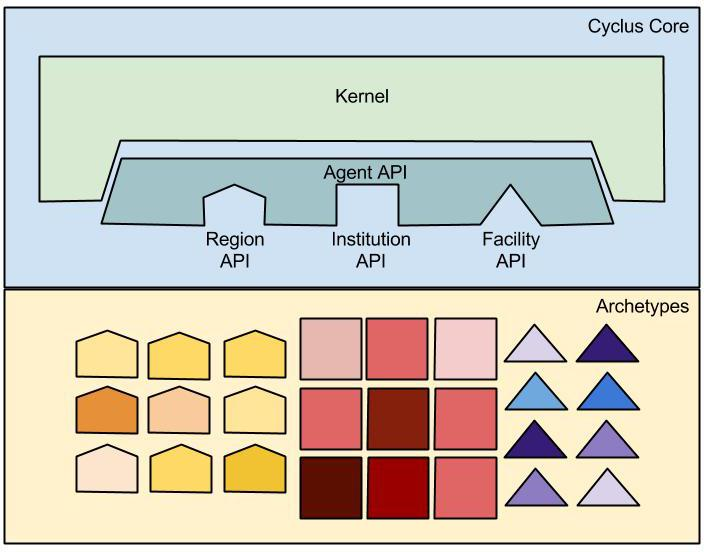
\includegraphics[width=\textwidth]{./images/framework}
\end{center}
\caption{The \Cyclus core provides \gls{API}s that abstract away the details in
the kernel and allow the archetypes to be loaded into the simulation in a modular
fashion.}
\label{fig:framework}
\end{figure}


An additional benefit is the ability for
contributors to choose different distribution and licensing strategies
for their contributions. Users and modelers control the accessibility of their archetypes and data sets (See Figure \ref{fig:modifiedopen}).
In particular, since the clean plug-in architecture loads libraries without any
modifications to the \Cyclus kernel, closed-source archetypes can be used with
the simulator alongside open source archetypes without transfer of sensitive information. This architecture
allows closed-source libraries (e.g., those representing sensitive nuclear
processes and subject to export control) to be developed and licensed privately.

\begin{figure}[htbp!]
\begin{center}
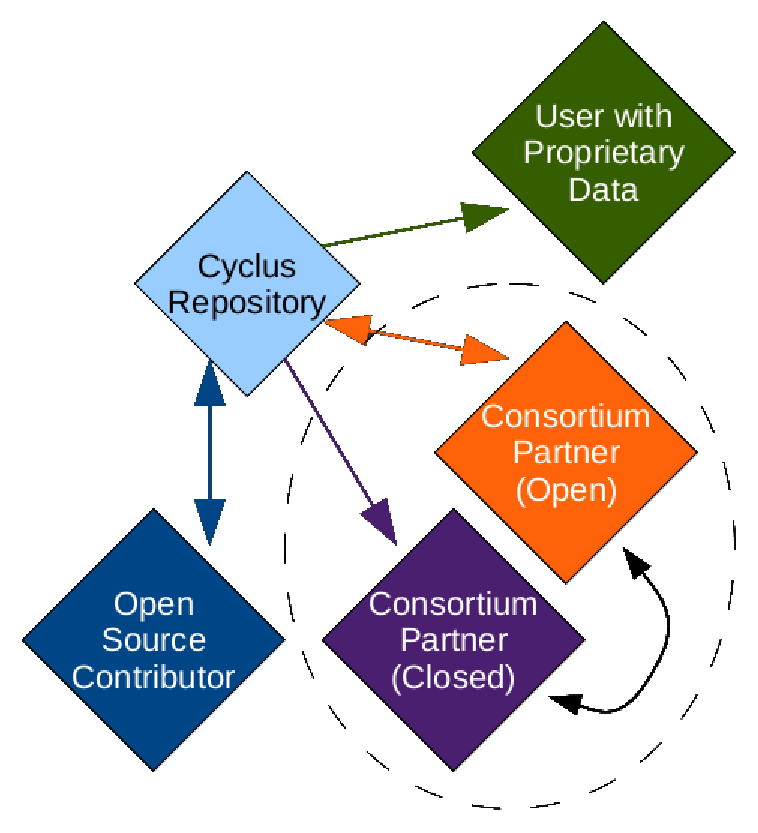
\includegraphics{./images/modifiedopen.eps}
\end{center}
\caption{The \Cyclus framework enables fully open, partially open, and fully
closed collaborations\cite{carlsen_cyclus_2014}.}
\label{fig:modifiedopen}
\end{figure}

Finally, dynamically loadable libraries enable \Cyclus to easily handle varying levels of simulation complexity. Hence a single
simulation engine can be used by both users interested in big-picture policy
questions as well as users focused on detailed technical
analyses. They merely choose their preferred level of modeling depth from among the
available libraries in the ecosystem.

\subsection{Agent-based Paradigm}
\label{sec:abm}
% superior detail in capturing simulation dynamics
% more flexible control over behavior
% describe Region/Institution/Facility hierarchy
% note importance of generic resource exchange paradigm

\Cyclus implements an \acrlong{ABM} paradigm. \gls{ABM} enables model
development to take place at an agent level rather than a system level. In the
nuclear fuel cycle context, for example, an analyst can design a reactor agent
that is entirely independent from a fuel fabrication agent. Defining the
behavior of both agents according to the
\gls{API} contract is sufficient for them to interact with one another as
bona fide agents in the simulation.  The two archetype libraries can be used in
the same simulation without any shared knowledge, allowing modelers to
construct a simulation from building blocks of many types and origins.

Furthermore, the \gls{ABM} paradigm is superior to the system dynamic approach used in
current simulators.
System dynamics is a popular approach for modeling nuclear fuel cycles
\cite{jacobson_vision_2009,van_den_durpel_daness_2009,guerin_impact_2009,guerin_benchmark_2009}.
Formally however, system dynamics models are simply a strict subset of agent-based models
\cite{macal_agent-based_2010}.
That is, any system dynamics model can be translated
into an agent-based model. Furthermore, because agent-based
techniques can provide a richer model than can system dynamics, they enable the
broadest range of simulations in a generic fashion.

\subsubsection{Agent Interchangeability}\label{sec:interchangeability}

% (OO, cpp, xml, backends, inheritances, mixins, generic apis, etc.)

\gls{ABM} is inherently object-oriented because agents represent discrete,
independently acting objects.  Figure \ref{fig:framework} illustrates the
modular nature of \Cyclus archetypes.  The core of the \Cyclus simulator creates
a set of classes on which agent plug-ins are based. In addition, a set of tools
are also provided to enrich the \gls{API} and supply a robust suite of behaviors
for the developer. Agent plug-ins utilize the generic core \gls{API} to
interact with one another.  For example, they use the resource exchange paradigm
\gls{API} for trading resources with one another.

Due to this plug-in architecture,
implementations of agents in a given scenario can be easily
interchanged. Critically, this novel functionality enables the comparison
between agent implementations. For example, a low-physics-fidelity
implementation of a reactor can be compared to an implementation with higher
physics fidelity, allowing an analyst to discern the effect of reactor physical
fidelity on a given fuel cycle.

Interchangeability is accomplished by providing \glspl{API} that define agent-to-agent
interaction and agent-to-environment interaction, primarily through the
\Class{Agent} and \Class{Trader} interfaces. Figure \ref{fig:agent_uml} shows
the ``inheritance'' structure of the \Class{Agent} class in a \gls{UML} diagram
format. It shows how the \Class{Agent} interface
provides a notion of parent-child hierarchical relationship, where parents can
choose to \textit{deploy} child agents and \textit{decommission} child
agents. For the archetype developer, this interface provides enormous power
very simply. The \gls{API} provides the \Class{Agent} with helpful functionality for
interacting with the \Cyclus simulation kernel while abstracting away unnecessary
detail.

\begin{figure}[htbp!]
\begin{center}
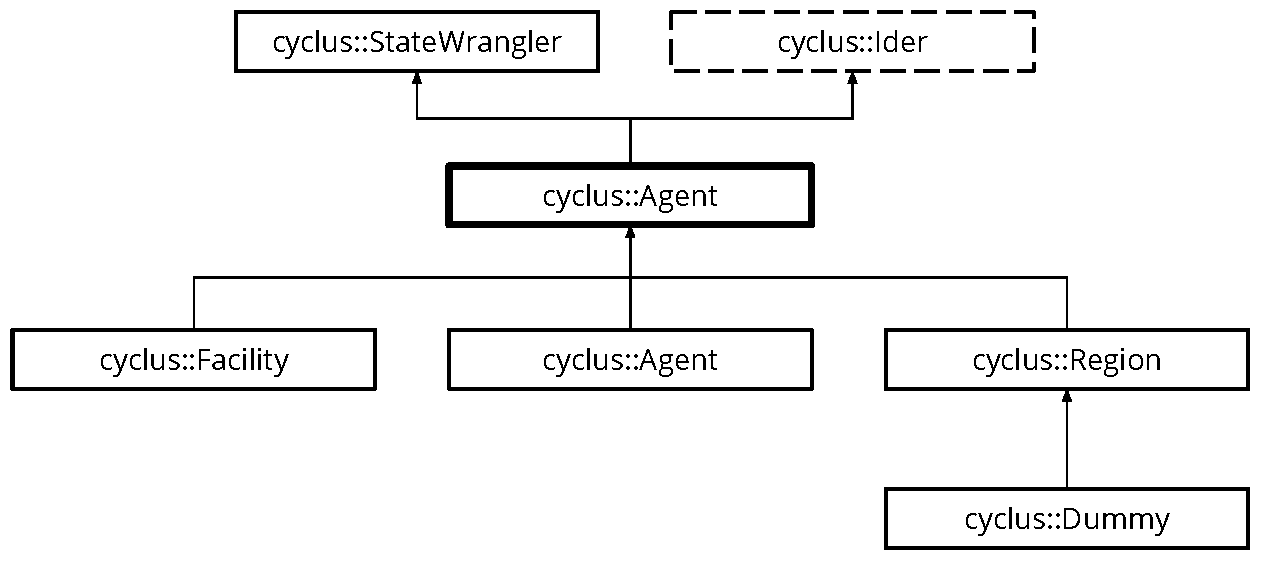
\includegraphics[width=0.5\textwidth]{./images/agent_uml}
\end{center}
\caption{The inheritance in \Cyclus classes, such as the \Class{Agent},
\Class{Facility}, \Class{Institution}, and \Class{Region} classes, abstract away
unnecessary details while exposing powerful functionality. In the above
example, the \Class{Dummy} archetype simply inherits from \Class{Region} in
order to become a bona fide Region-type \Class{Agent}.}
\label{fig:agent_uml}
\end{figure}

In this way, a researcher can directly compare two different reactor modeling
implementations (perhaps the imaginary classes \Class{DetailedReactor} and \Class{SimpleReactor})
simply by exchanging the two corresponding archetypes. That is, two reactor
archetypes both inheriting from the \Class{Facility} class are indistinguishable
from a simulation perspective.  This can be done with any agent type, where agents can be ``Regions,'' ``Institutions,'' or ``Facilities.''

\subsubsection{Regions, Institutions, and Facilities}

\Cyclus provides a novel representation of entities in the nuclear fuel cycle
that reflects the reality in international nuclear power: facilities implementing individual fuel cycle technologies, institutions managing those facilities, and regions providing geographical and political context for institutions and facilities. While
few simulators have provided any notion of static regional
effects \cite{huff_next_2010,juchau_modeling_2010}, \Cyclus allows for both regions and institutions to be first-class
agents in simulated fuel cycles. The fundamental interactions for each entity are implemented in a corresponding
archetype class in \Cyclus, i.e., the \Class{Region} class, \Class{Institution}
class, and \Class{Facility} class. Archetype developers can then build on the
provided functionality by inheriting from the appropriate class.
\Cyclus implements a \gls{RIF} relationship through the
parent-child hierarchy described in \S \ref{sec:interchangeability}, where
regions are the parents of institutions which are, in turn, the parents of
facilities. In other words, \gls{RIF} hierarchies form a directed acyclic graph (DAG),
with regions as root nodes and facilities as leaf nodes.

Two primary consequences arise from this structure. First, institutions are
nominally responsible for deploying and decommissioning facilities. Accordingly, advanced
logic regarding building and decommissioning can be implemented on top of
those behaviors inherited from the
\Class{Institution} interface. Second, the \Class{Facility} class implements the
\Class{Trader} interface, and thus institutions and regions, respectively, can
adjust the resource flow preferences of their managed facilities. Importantly,
this capability allows for the modeling of preferential regional trading
of resources (e.g., tariffs) as well as preferential institutional trading
(e.g., long-term contracts).

\subsection{Discrete Objects}
% enables more realistic models and metrics
% material routing metrics
% shadow fuel cycles
% etc.

\Cyclus models facilities, institutions, regions, and resources as discrete
objects. A discrete resource model allows for a range of modeling granularity. In the
macroscopic extreme, it is equivalent to time-stepped continuous flow. In the
microscopic extreme, the model is capable of representing arbitrarily small
material objects at isotopic resolution. In this way, \Cyclus is
applicable across the full range of modeling fidelity.

Fleet-based, lumped-material models do not distinguish between discrete facility
entities or materials. However, some questions require resolution at the level
of individual facilities and materials.  As a result, many detailed performance
metrics cannot be captured with previously existing fleet-based models. For all
of the reasons that the \gls{ABM} paradigm in \ref{sec:abm} enables novel
simulations, multiple use cases require that these agents, such as the regions,
institutions, and facilities in \Cyclus, must be represented as discrete
objects. For instance, tracking of individual shipments is only viable if materials and
resources are tracked as discrete objects.

\subsubsection{Resources and Materials}
% Resources, Materials (note isotope tracking, decay behavior)

Another such use case seeks to capture system vulnerability to
material diversion. Provenance and trade-history of distinct materials is the fundamental
information unit in such studies, and so this type of analysis requires
 discrete simulation of a
target facility and the individual materials modified within it.
Material risk analysis, therefore, demands that both facilities and materials
should be discretely modeled objects like those in \Cyclus.

In \Cyclus, agents can transfer discrete resource objects among one another.
Cyclus supports two types of resources:

\begin{itemize}

  \item materials: these represent typical nuclear materials with
      nuclide compositions;

  \item products: these can represent any user-defined measure: carbon
      credits, build permits, employees, etc..

\end{itemize}

All operations performed on every resource object (splitting, combining,
decay, etc.) are tracked in detail as they are performed.  This information
includes the agent that created each resource when it was introduced into the
simulation.  The parentage of each resource is also tracked. This makes it
possible to follow the history of resources as they are transferred between
agents.

The \Cyclus kernel has built-in experimental support for decay calculations.
Materials store the time since their last decay and agents are free to
invoke the decay function on them as desired to decay them to the current
simulation time. \Cyclus can currently operate in 3 decay modes, with 1 additional
mode likely to be added in a future release:

\begin{itemize}

    \item "manual" (currently implemented) is the default mode
        where agents decay materials as needed,

    \item "never" (currently implemented) globally turns off all decay.
        The Material decay function does nothing,

    \item "lazy" (currently implemented) decays any material whenever its
        composition is observed (e.g. when an agent queries information about
        a material's $^{239}$Pu content),
    \item "periodic" (future) automatically decays all materials in a
        simulation with some fixed frequency.

\end{itemize}


When decay is invoked, a material checks to see if it contains any nuclides with
decay constants that are significant with respect to the time change since the
last decay operation.  If none of the decay constants are significant, no decay
calculation is performed and the material remains unchanged.  This error does
not accumulate because the next time the material's decay function is invoked,
the time change will be larger.

\Cyclus has no notion of ``tracked'' versus ``untracked'' nuclides.  In
\Cyclus, the composition of a material is represented by an arbitrarily large
list (potentially thousands) of nuclides.  Agents are free to treat nuclides
present in materials any way they please - including ignoring them.  It is the
responsibility of archetype developers to choose how to handle potentially
full-fidelity compositions.

In large simulations, many material objects may change frequently.  Material
decay can also contribute significantly to such changes.  In order to help
avoid unnecessary runtime performance and database size impacts, compositions
in \Cyclus have some special features.  In particular, compositions are
immutable once created. This allows multiple material objects to hold
references to the same composition safely.  Additionally, new compositions
resulting from decay are cached and used to avoid redundant decay
calculations.  Figure \ref{fig:compositions} illustrates how this decay
history cache works. Composition immutability in concert with decay history
caching help eliminate many redundant calculations in addition to reducing the
total number of composition entries recorded in the database.


\begin{figure}[htbp!]
\begin{center}
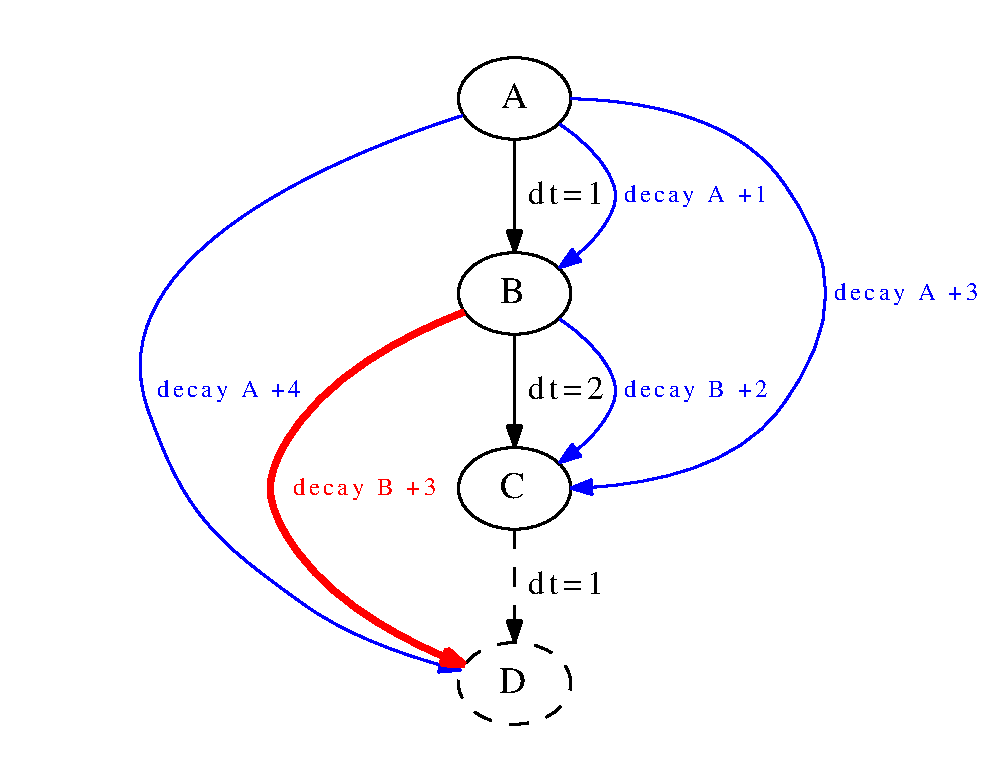
\includegraphics{./images/compositions}
\end{center}
\caption{
A simple decay line cache holding compositions A, B, C, and a
yet-uncomputed composition D.  B comes from decaying A 1 time step.  C comes
from decaying B 2 time steps, etc.  Black represents the cache for this
particular composition chain. Blue indicates decay operations that can be
satisfied by cache lookups.   If A needs to be decayed 1 time step (A +1), a
quick lookup returns the previously computed B.  Decaying B 3 time steps
requires a decay calculation to compute a new composition D, but subsequent
requests such as decaying A 4 time steps will not require any recalculation.
}
\label{fig:compositions}
\end{figure}

% although this abbreviation is provided by the glossary capability, I think
% the DRE is so important that it should be redefined here.

\subsubsection{Dynamic Resource Exchange (DRE)}

The \Cyclus simulation paradigm allows discrete agents, based on archetypes
about which the kernel has no knowledge, to enter the simulation at arbitrary
times and trade in discrete resources. These resources are not defined \textit{a
  priori}. Therefore, the logic engine defining resource interaction mechanisms
among agents is crucial. The \gls{DRE} is that critical logic engine on which
\Cyclus simulations are built.  Supporting the general \Cyclus philosophy,
facilities are treated as black boxes and a supply-demand communication
framework is defined.

The \gls{DRE} consists of three steps: supply-demand information
gathering, resource exchange solution, and trade execution. Importantly, each
step is agnostic with respect to the exchange of resources in question, i.e.,
the same procedure is used for both Materials and Products.

The information-gathering step begins by polling potential consumers. Agents
define both the quantity of a commodity they need to consume as well as the
target isotopics, or quality, by posting their demand to the market exchange as
a series of \textit{requests}. Users may optionally parameterize the agent to
associate a collection of demand constraints with each collection of requests.
Collections of requests may be grouped together, denoting \textit{mutual}
requests that represent demand for
some common purpose. For example, a reactor may request \gls{UOX} and \gls{MOX} fuel
mutually, indicating that either will satisfy its demand for fuel.

Suppliers then respond to the series of requests with a \textit{bid}. A bid
supplies a notion of the quantity and quality of a resource to match a
request. Suppliers may add an arbitrary number of constraints to accompany
bids. For example, an enriched \gls{UOX} supplier may be constrained by its current
inventory of natural uranium or its total capacity to provide enrichment (SWUs), and
attach such constraints to its bids.

Any potential resource transfer, i.e., a bid or a request, may be denoted as
\textit{exclusive}. An exclusive transfer must either be met fully or not at all
in order to support concepts such as the trading of individual reactor
assemblies.  In combination with the notion of mutual requests, complex instances
of supply and demand are enabled.

Finally, requesting facilities, institutions and regions may apply
\textit{preferences} to each potential request-bid pairing based on the proposed
resource transfer. Facilities can apply arbitrary complex logic to rank the bids
that they have received, whether based on the quantity available in each bid or
on the quality of each bid, and the consequent implications of the physics behavior
of that facility. In addition, an institution can apply a higher preference to a
partner to which it is congenial; similarly, a region may negate any transfers
of material which have a higher uranium enrichment than is allowable.

Given a full definition of supply and demand, the \gls{DRE} may be solved either
optimally using a mathematical program or approximately by a simulation-based
heuristic \cite{gidden_agent-based_2014}. If any trade is denoted as exclusive, e.g., if an
analyst desires an assembly-fidelity model, then either a heuristic must be used
or exchanges must be represented as a \gls{MILP}. If no exclusive trades exist,
a \gls{LP} model may be used. In practice, LPs solve much faster than
\gls{MILP}s. However, both capabilities exist in \Cyclus in order to
provide users with the desired level of fidelity.

Trades between agents are initiated by the \Cyclus kernel after a solution to
the \gls{DRE} is found. For each trade, the supplying agent is notified of its
matched request and provides an associated resource to the exchange. All
supplied resources are then sent to the corresponding requesting agents.

In \Cyclus, the \gls{DRE} is executed at each time step. Therefore, if a
facility's request for a resource is not met at a given time step, it may offer
a request in the following time step. Because agent behavior may change
arbitrarily, the exchange executed at any given time step may be unique in a
simulation.

The \gls{DRE} is a novel simulation concept in the nuclear fuel cycle domain. It
provides a flexible supply-demand infrastructure, supporting dynamic flows of
resources between agents, even as those agents enter and leave the simulation, and
even when those agents are defined by archetypes of arbitrary complexity. Trading
between agents can be affected by both the
proposed quality of a resource and agent relationships through the use of
preferences. Accordingly, a wide range of possible effects can be
modeled, from capacity-limited fuel supply to international trade agreements.

\subsection{Simulation Support}
So that users and developers can build working simulations in the shortest time
possible, the \Cyclus ecosystem provides fundamental building blocks: basic
archetypes and a toolkit of commonly needed functions.  The \Cycamore library
provides a suite of fundamental Region, Institution, and Facility archetypes,
while the \Cyclus toolkit provides assistance to developers.

\subsubsection{Cycamore}
% base modules

\Cycamore \cite{carlsen_cycamore_2014}, the \Cyclus additional module
repository, provides a fundamental set of agent archetypes for basic simulation
functionality within \Cyclus.  Since \Cyclus relies on external
archetypes to represent the agents within a simulation, \Cycamore provides the
basic archetypes a new user needs to get started running simple simulations.
These archetypes support a minimal set of fuel cycle simulation goals and
provide, by example, a guide to new developers who would seek to contribute
their own archetypes outside of \Cycamore.

As of version 1.0, \Cycamore contains one region archetype, two institution
archetypes, and four facility archetypes. Short descriptions of these functions
can be found in Table \ref{tab:cycamore}.


\begin{table}[h]
\centering
\begin{tabularx}{\textwidth}{|r|l|X|}
\hline
\textbf{Entity} & \textbf{Archetype} & \textbf{Functionality} \\
\hline
Facility & BatchReactor & A reactor model that handles batch refueling, based on pre-determined recipes of compositions. \\
Facility & Source & This facility generates material of the composition and commodity type specified as input.  \\
Facility & Sink & This facility is capable of accepting a finite or infinite quantity of some commodity produced in the simulation. \\
Facility & EnrichmentFacility & This facility enriches uranium at a specified capacity. \\
Institution & ManagerInst & The manager institution manages production of commodities among its facilities by building new ones as needed. \\
Institution & DeployInst &  This institution deploys specific facilities as defined explicitly in the input file. \\
Region & GrowthRegion & This region determines whether there is a need to meet a certain capacity (as defined via input) at each time step. \\
\hline
\end{tabularx}
\caption{The Archetypes in \Cycamore seek to cover a large range of simple simulation use cases \cite{carlsen_cycamore_2014}.}
\label{tab:cycamore}
\end{table}

As illustrated in
Figure \ref{fig:simplesim}, the current \Cycamore release provides basic
functionality enabling simple fuel cycle analyses. As future contributions are
vetted, the capabilities in \Cycamore may grow.

\begin{figure}[htbp!]
\begin{center}
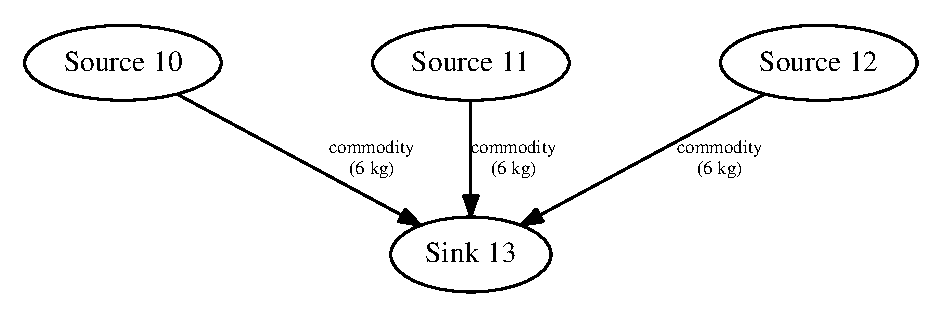
\includegraphics{./images/simplesim}
\end{center}
\caption{Material flows through a simple dynamic simulation created with only the simplest \Cycamore archetypes, \Class{Sink} and \Class{Source}.}
\label{fig:simplesim}
\end{figure}

\subsubsection{Toolkit}

In addition to the core functionality of the \Cyclus kernel, which is focused on
the set of capabilities needed to implement an agent-based simulation
with \gls{DRE}, a toolkit is provided to assist developers
and users with related simulation and nuclear engineering tasks. The toolkit is
an actively developed part of \Cyclus, with a primarily forward-looking
focus on supporting interesting \textit{in situ} metric analysis tools.

\paragraph{Simulation Tools}

A series of utility classes are provided to support demand-constrained agent
facility deployment. For example, symbolic function representations of linear,
exponential, and piecewise functions are supported via the
\Class{SymbFunctionFactory} class. Such functions are used with other toolkit
classes to determine commodity demand (e.g., power demand) from user input. Four
mix-in classes provide the basis for in-simulation deployment determination:
\Class{CommodityProducer}, \Class{CommodityProducerManager}, \Class{Builder},
\Class{BuildingManager}. The \Class{CommodityProducer} class provides an
interface for querying the \textit{prototypes} which have the
capacity to produce a given commodity. The \Class{CommodityProducerManager}
provides an interface for registering \Class{CommodityProducer}s and querying
the current capacity (supply) of a commodity. The \Class{Builder} class provides
an interface for querying which prototypes can be built and interacts with the
\Class{BuildingManager}, which orders prototypes to be built. The
\Class{BuildingManager} uses a simple minimum cost algorithm to determine how
many of each prototype, $y_i$, to build given a demand ($\Phi$), capacities
($\phi_i$), and costs ($c_i$). Here $i$ indexes $I$ available prototypes which perform a similar function, and the demand, capacity and cost carry prototype-specific units which are defined by the developer.

\begin{equation}
\begin{aligned}
 \min & \sum_{i=1}^{N}c_i y_i \\
 s.t. & \sum_{i=1}^{N}\phi_i y_i \ge \Phi \\
      & y_i \in [0,\infty) \:\: \forall i \in I, \:\: y_i \:\: \text{integer}
\end{aligned}
\end{equation}

\paragraph{Nuclear Engineering Tools}

The \Cyclus toolkit provides two useful interfaces for querying physical parameters of \Class{Material}
objects. First, the \Class{MatQuery} module
provides a basic querying \gls{API}, including the atom and mass fractions of
nuclides, the number of moles of a nuclide in a material, and also the amount of
aggregate nuclides, i.e., a \Class{Composition}, in a material. The
\Class{Enrichment} module provides an \gls{API} for determining enrichment-related
parameters of a material, including the separative work units (SWU) and natural
uranium required to enrich a material provided knowledge of feed, product, and tails
assays.

\paragraph{Toolkit Extensions}

In addition to those that already exist, new tools will
emerge from the archetypes developed by the community. As these tools gain adoption between projects and demonstrate their
utility to the developer community, they will be considered for screening and
adoption into the kernel as toolkit extensions. Likely extensions include

\begin{itemize}
\item fuel cycle metrics calculators,
\item supportive data tables,
\item policy models,
\item and economic models.
\end{itemize}

\subsection{Quality Assurance}
% Organize this section according to major topics
% give each topic a section heading in boldface.
% try to cover the major common points :
%
% problem design
% methods of measurement
% supporting models
% supporting data
% simulations run
% results

% Just write the section headings for each part and indicate what goes in that
% section with words :
%
% heading
% figures (with captions)
% schematics (with captions and footnotes)
% equations
% tables

% What does it mean?
% What did I actually test?
% What were the results?
% Did the work yield a new method?
% Did the work yield new knowledge?
% What measurements did I make?
% How were these measurements characterized?
% What methods were used?
% What were the results?
% How were the measurements made and characterized?

Simulation science - like experimental science - must distinguish trustworthy
results from untrustworthy ones.
Charles Babbage famously articulated this, ``On two occasions I have been asked,
`Pray, Mr. Babbage, if you put into the machine wrong figures, will the right
answers come out?' ... I am not able rightly to apprehend the kind of confusion
of ideas that could provoke such a question.'' \cite{babbage_passages_2011}.
A simulator must assure correctness and guard against the \emph{garbage
in, garbage out} phenomenon.

Multiple strategies, collectively known as \emph{\gls{QA}}, have
been invented to mitigate structural and algorithmic errors
in software. These include \emph{\gls{VV}}
\cite{boehm_software_1989}, \emph{\gls{UQ}}
\cite{sacks_design_1989}, testing, and others.

Nuclear engineering software quality is often governed by \gls{NQA1}, an
\gls{ASME} specification
whose latest revision appeared in 2009 \cite{asme_nqa-1a-2009_2009}.
\Cyclus has adopted an \emph{agile} development process
\cite{larman_agile_2004},
interpreting \gls{NQA1} in a manner similar to the process adopted by the
\gls{DOE} within \gls{NEAMS} \cite{neams_nuclear_2013} or by the PyNE toolkit
\cite{biondo_quality_2014}.

Since \Cyclus modeling decisions are made
by third party archetype developers or users, the most important feature of
\gls{QA} is verification. Validation of the \Cyclus core in a general sense is infeasible as it is contingent on the archetypes comprising a simulation, and to be meaningful \gls{UQ} must likewise extend beyond the kernel.

Verification may be defined as the question, ``Is \Cyclus being built correctly?''
To answer this question, \Cyclus relies on software development best practices
such as testing,
documentation, version control, style guidelines, and continuous integration to
ensure reliability and reproducibility. These verification techniques are
discussed individually in the sections that follow.

Validation, in contrast,  may be defined as the question,
``Is \Cyclus the correct tool?''
Since \Cyclus is alone in its class as an agent-based fuel cycle simulator, longitudinal
validation is not possible. Nonetheless, code-to-code comparisons with fuel cycle
simulators that use other modeling paradigms are underway
\cite{huff_extensions_2014}. However, such
exercises are more likely to bring into relief the differences between the modeling
paradigms than supply substantial \gls{QA} and validation.

Lastly, \gls{UQ} is a process that is used on specific simulation
instantiations to statistically determine quality. \gls{UQ} is a process that applies
to the running of many \Cyclus simulations. The kernel itself, as a generic fuel cycle
simulator, cannot make reliable statements about the uncertainty of metrics for a particular fuel
cycle. Any \gls{UQ} results are applicable only to the scenario that is under
analysis by the user. \Cyclus is not a substitute for due diligence on behalf of the fuel
cycle modeler. Thus, \gls{UQ} is envisioned to be beyond the scope of core development
and in the domain of the expert user.

Sections \ref{sec:qa-testing}-\ref{sec:qa-ci} discuss in greater detail the software
development components that comprise the \Cyclus verification strategy.
Each of these on its own is a valuable addition to \gls{QA} but is cannot be the
entire answer to the requirements imposed by \gls{NQA1}. Taken together and strictly
adhered to, they present a fortress to protect against poorly designed or otherwise undesirable code.


\subsubsection{Testing}
\label{sec:qa-testing}

Automated software \emph{testing} is the first line of defense against
errors in implementation. It also acts as an early warning sign if the
simulator does not work as intended on a new system.
Testing serves a critical role in \gls{QA} because it directly compares the
results of running software versus the expected behavior of the software.
In \Cyclus, three categories of tests are defined: unit tests, integration
tests, and regression tests.

It is important to note that before a proposed
code change is allowed into \Cyclus,  the change must be covered by a test, either new or existing, and all tests must pass.  Of course, test code is
just as likely to contain errors as the code it is designed to test.
However, it is assumed that diligence and one level of testing
is sufficient to meet the aims of \gls{QA} and prevent an infinite recursion
of testing-the-tests.

\paragraph{Unit Tests}

Unit tests compare the results of the smallest code \emph{unit},
typically a single function or a class. What constitutes the smallest code
unit depends on the context of the specific unit in question. While this is
an ambiguous definition, when combined with a philosophy of keeping units as small
as possible, it is often clear in practice what needs to be tested.

\Cyclus uses the Google Test framework \cite{inc_googletest_2008} as a harness for running unit
tests. Sufficient unit tests are required for any proposed change to the \Cyclus
code base. Currently, \Cyclus implements over 450 unit tests and \Cycamore implements
85.  These cover approximately 65\% of their respective code bases, and these numbers are expected to grow over time.

\paragraph{Integration Tests}

Integration tests combine multiple elements of the
\Cyclus interface and test that they work correctly with each other.  By analogy,
simply because the gears (units) are made correctly does not imply that the
clock (integration) will run smoothly, run at all, or give the correct time.
In \Cyclus and \Cycamore, integration tests are performed by running sample
simulations for scenarios that are sufficiently simple to predict the results and verifying
        that results match those predictions. A set of standard input files have thus been constructed.
Python is used to run the same set of \Cyclus simulations as a subprocess for each integration test.
 The results are then inspected and compared via Nose \cite{pellerin_nose_2007}, a Python test framework.
In this way, \Cyclus code units are tested in the full context that they will be
executed. This category of testing is especially useful for ensuring that
major \Cyclus components are functioning as expected.

\paragraph{Regression Tests}

Regression tests ensure significant unintended changes do not
occur over the course of \Cyclus development. Such a change is called a
\emph{regression} because the new version is almost always wrong.
Regression tests are implemented similarly to integration tests.
Nose is used to execute full \Cyclus simulations whose results
are then compared. In this category, however, the comparison is done against
the output of the same input file when run with a previous version of \Cyclus,
typically the last released version.
In some sense, regression tests are `dumb' in that they do
not care about the contents of a simulation being correct, only whether or not
it changed. They pick up glaring time-sensitive mistakes that may
not appear elsewhere, though they do not purport to make claims about the
quality of the physics modeled. Regression tests are primarily implemented
in \Cycamore because its archetypes are sophisticated enough
to make interesting simulations.

\subsubsection{Documentation}

All of the public interface (the \gls{API}) must be documented as required by the \Cyclus
\gls{QA} policy. This certifies that the intention for a code unit is communicated
in way that is separate from its implementation. This policy is important
because implementations are often wrong and do not reliably communicate their intent. Truly trustworthy communication about what
software should be doing occurs when the author explicitly states the
goals of an \gls{API} in prose form. Future developers are then able to
compare the implementation versus the documentation to discern whether or not
these are in agreement. Documentation is thus a secondary higher-level information
stream.  In \Cyclus, this information is aggregated together into static
websites with the Doxygen \cite{van_heesch_doxygen:_2008} and Sphinx
\cite{brandl_sphinx_2014}
tools, and can be accessed at \url{http://fuelcycle.org}.

\subsubsection{Version Control}

Version control preserves the development history, or \emph{provenance}, of
source code files. \Cyclus uses a well-established \emph{distributed version
control} tool called git \cite{software_freedom_conservancy_git_2014} for this
purpose.  Distributed version control allows every
user to have complete local copy of the \emph{repository} (the version control
term for the collection of all possible histories).
One feature that git performs exceptionally well is \emph{branching}.
Branches are distinct pathways in the history that diverge from a mainline source
tree and then may be \emph{merged} back in. Multiple simultaneous
branches may exist at all points in time. Every change to the code is recorded
in the history, along with metadata such as the author, a timestamp, and an
accompanying message. Thus,
it is possible for \Cyclus to accurately replay the entirety of who did what to the
code when.

\Cyclus uses a strategy known as \emph{git flow}
\cite{kalliamvakou_code-centric_2014} to manage topical branches where
individuals develop code in parallel. All proposed software changes from
topical branches must have sufficient successful tests and comprehensive
documentation to be allowed into \Cyclus.  As an example, a schematic of the
development stages between reporting a bug and merging the fix is shown in
Figure \ref{fig:gitprocess}.

\begin{figure}[htbp]
\begin{center}
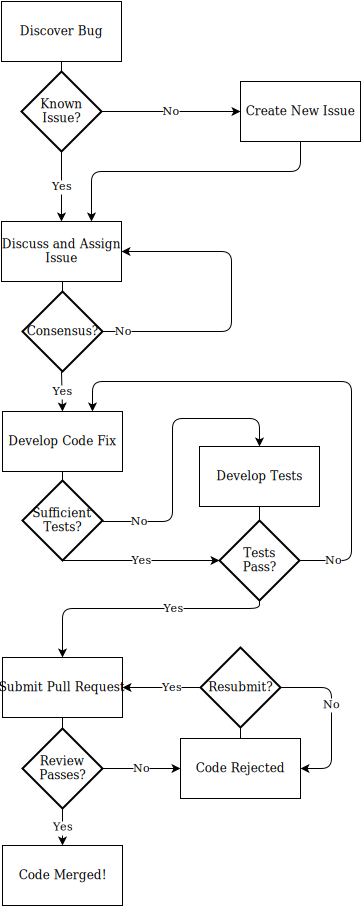
\includegraphics[height=0.6\textheight]{./images/gitprocess}
\end{center}
\caption{A version-control enabled process for finding, reporting, and fixing a bug
can take place within an issue tracker alongside multiple stages of software
testing and review. In the \Cyclus case, the final review stage includes unit,
regression, and integration testing as well as manual code inspection.}
\label{fig:gitprocess}
\end{figure}

The act of proposing a change is known as a \emph{pull request}. The main \Cyclus repository is
hosted remotely on the GitHub website \cite{dabbish_social_2012}. The online
mechanism for pull requests allows for code review by a member of the \Cyclus
core team, separate from the author, prior to any change being included. Non-members
of the \Cyclus development team are allowed and encouraged to submit and review
pull requests. However, only members of the \Cyclus core team are allowed to
merge in any changes and only after the \gls{QA} standards have been met. This
step has been repeatedly shown to improve code quality \cite{cohen_modern_2010}.

\subsubsection{Style Guide}

In any multi-person software project, there is a tension between how individuals
wish to write code. Every person tends to have their own custom style. To remedy this,
coding style guides are the software analogy to those for written language,
such as the Chicago Manual of Style. \Cyclus strictly enforces the use of the
Google C++ Style Guide \cite{weinberger_google_2008} for all software contributions.
This means that all developers of \Cyclus nominally write \Cyclus code in the same
way.  This homogenization may be a hurdle to new developers but ultimately
improves code legibility and, therefore, robustness \cite{cohen_modern_2010}.

\subsubsection{Continuous Integration}
\label{sec:qa-ci}

\emph{\acrfull{CI}} is the idea that software should be tested and validated
as it is being developed, rather than as a final stage in a longer development
cycle.  Under \gls{CI}, every pull request (proposed code change) is tested independently immediately after
it is proposed. Such tests are run on all officially supported platforms.
\Cyclus uses a \gls{CI} platform called Polyphemus
\cite{scopatz_polyphemus_2014}. Polyphemus serves as an intermediary between GitHub pull requests on the front-end
and temporary \Cyclus servers on the back-end. These servers are hosted by
the Build \& Test Laboratory (BaTLab) \cite{uw_batlab_team_batlab_2014} at the University of
Wisconsin-Madison. Whenever a pull request is created, Polyphemus performs
the following actions:

\begin{enumerate}
    \item Copies \Cyclus with the proposed new code to BaTLab,
    \item Initializes Linux and Mac OSX servers,
    \item Builds \Cyclus on all platforms,
    \item Runs the complete \Cyclus test suite,
    \item Reports whether or not the above steps succeeded.
\end{enumerate}

Since these steps are performed for all incoming code, it is easy for the
\Cyclus core team to determine whether or not an individual pull request
actually works. This helps identify build and test problems prior to
broken code being allowed into the develop branch. \gls{CI} is a necessary
but not sufficient addition to the \Cyclus \gls{QA}
system: it keeps bad code out of \Cyclus. However, \Cyclus will always
require human eyes and hands to let good code in.

\section{Examples}
% Organize this section according to major topics
% give each topic a section heading in boldface.
% try to cover the major common points :
%
% problem design
% methods of measurement
% supporting models
% supporting data
% simulations run
% results

% Just write the section headings for each part and indicate what goes in that
% section with words :
%
% heading
% figures (with captions)
% schematics (with captions and footnotes)
% equations
% tables

% What does it mean?
% What did I actually test?
% What were the results?
% Did the work yield a new method?
% Did the work yield new knowledge?
% What measurements did I make?
% How were these measurements characterized?
% What methods were used?
% What were the results?
% How were the measurements made and characterized?

\subsection{Ecosystem}
% Cycamore library
% Cyder?

The archetypes created by user-developers and the archetypes provided in the 
\Cycamore \cite{carlsen_cycamore_2014} repository of additional modules 
together form an `ecosystem' of capabilities. Since the long term vision for 
the \Cyclus framework includes an ever-expanding ecosystem of both general and 
specialized capability extensions within that ecosytem. The early growth and 
cross-institutional contributions to this ecosystem demonstrates a significant 
acheivement by the \Cyclus framework. 

\subsubsection{The Cyclus Additional Modules Repository}

\Cycamore, the \Cyclus additional modules repository, provides a fundamental 
set of agent archetypes for basic simulation functionality within \Cyclus.
Since the \Cyclus framework relies on external archetypes to represent the 
agents within a simulation, 
\Cycamore provides the basic archetypes a new user needs to get started running 
simple simulations. 
These archetypes support a minimal set of fuel cycle simulation goals and 
provide, by example, a guide to new developers who would seek to contribute 
their own archetypes outside of \Cycamore.

\subsubsection{External Modules}
External modules have been 
\cite{cyder,separations,streamblender,mktdriveninst,commodconverter} and are 
being \cite{britelite,utk} developed for contribution to the cyclus ecosystem 
of models. 



\subsection{Simulations}
%FCO example (will be done soon.. publishable?)
%Inpro example (is this still running or did we deprecate it with 1.0?)

% MJG - INPRO should be tried again. @rwcarlsen has been running lots of
% simulations with the batch reactor, and its the second generation of my
% reactor models. We could easily use the same demand schedule and enrichment
% facility parameters and run it again.

Simulations have been run in the past and more are being run. FCO is an 
example. 

Some simple examples of recycle scenarios in \Cyclus follow.  In \Cyclus,
because material is tracked as discrete objects, single-pass mox recycle is
easy to implement.  The \textit{BatchReactor} archetype from \Cycamore has the
ability to accept fuel from multiple input sources with non-uniform
preference.  The dynamic resource exchange makes it easy for a reactor to
preferrentially accept recycled MOX fuel over fresh UOX fuel.  The material
flows for this simulation are shown below in figure \ref{fig:flow-modopen}.

\begin{figure}[!]
\label{fig:flow-modopen}
\caption{Modified open 1-pass MOX recycle fuel cycle material flows.}
\begin{center}
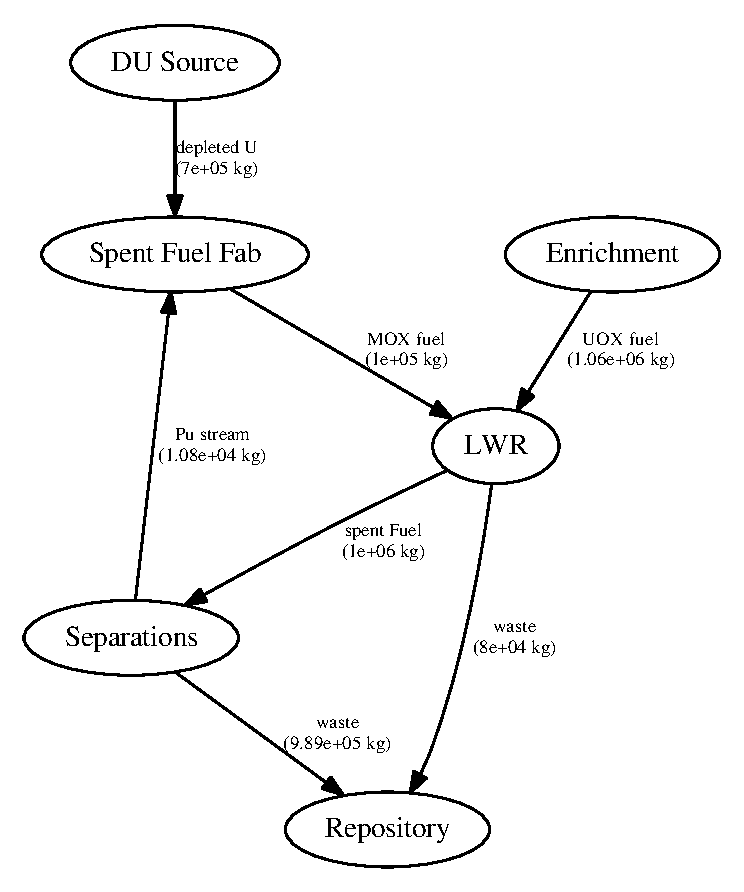
\includegraphics{./images/flow-mod-open-1.eps}
\end{center}
\end{figure}

To switch to a fully closed fuel cycle, all that needs to be done is change
the output commodity for the \textit{BatchReactor}'s spent MOX fuel.  All this
requires is a single word change in the input file resulting in the material
flows in Figure \ref{fig:flow-closed}.  Note that because the
\textit{BatchReactor} always transmutes fuel into the same composition, the
nuclide level flows are not realistic for the full, multipass recycle case.

\TODO{mention how fuel fab mixes fissile and filler streams}

\begin{figure}[!]
\label{fig:flow-closed}
\caption{Full MOX recycle (multi-pass) fuel cycle material flows.}
\begin{center}
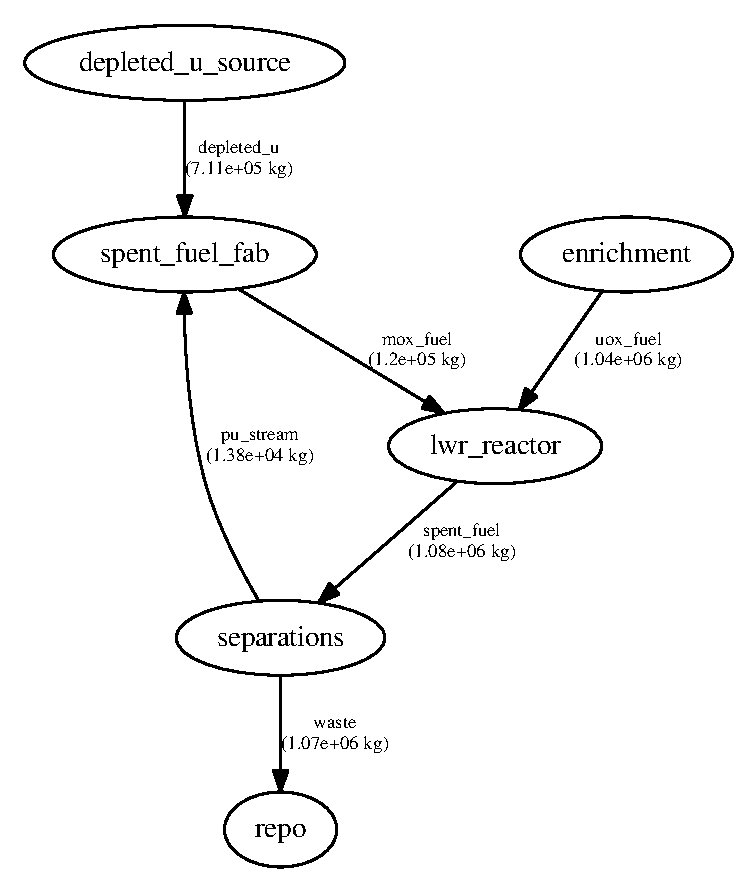
\includegraphics{./images/flow-closed-1.eps}
\end{center}
\end{figure}

\TODO{discuss Pu buildup charts}

\begin{figure}[!]
\label{fig:puseries-1}
\caption{bla}
\begin{center}
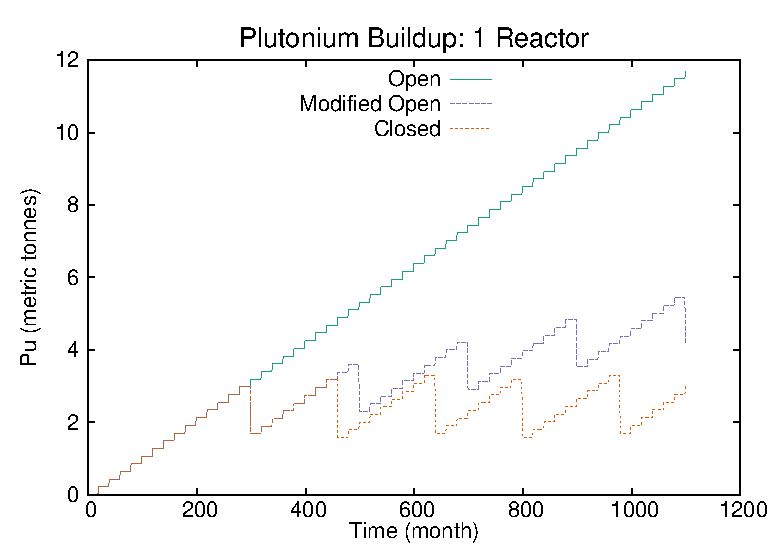
\includegraphics{./images/puseries-1.eps}
\end{center}
\end{figure}

\begin{figure}[!]
\label{fig:puseries-n}
\caption{bla}
\begin{center}
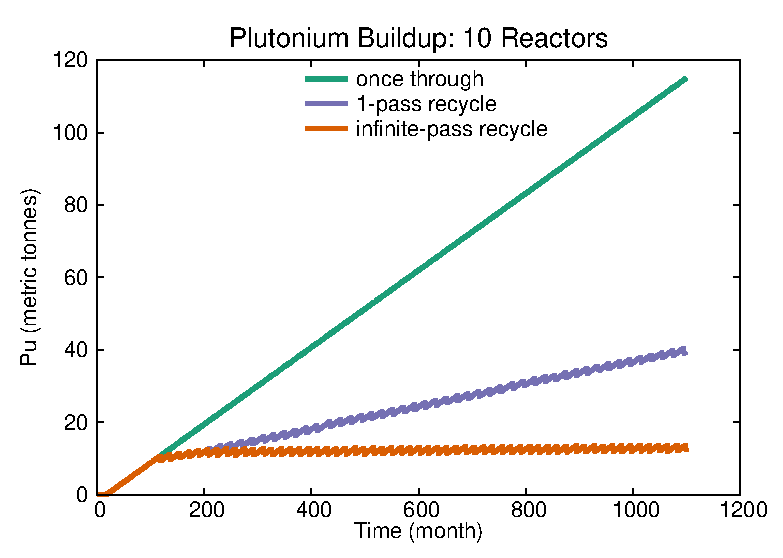
\includegraphics{./images/puseries-n.eps}
\end{center}
\end{figure}


\section{Quality Assurance}
% Organize this section according to major topics
% give each topic a section heading in boldface.
% try to cover the major common points :
%
% problem design
% methods of measurement
% supporting models
% supporting data
% simulations run
% results

% Just write the section headings for each part and indicate what goes in that
% section with words :
%
% heading
% figures (with captions)
% schematics (with captions and footnotes)
% equations
% tables

% What does it mean?
% What did I actually test?
% What were the results?
% Did the work yield a new method?
% Did the work yield new knowledge?
% What measurements did I make?
% How were these measurements characterized?
% What methods were used?
% What were the results?
% How were the measurements made and characterized?

Simulation science - like experimental science - has since the begining had the 
problem of identifying trustworthy results from the nonsensical and the noise.
This is epitomized in the Charles Babbage quote, ``On two occasions I have been asked, 
`Pray, Mr. Babbage, if you put into the machine wrong figures, will the right 
answers come out?' ... I am not able rightly to apprehend the kind of confusion 
of ideas that could provoke such a question.'' \cite{babbage_passages_2011}. 
The \emph{garbage in, garbage out} phenomenon is not the only scenario which a
simulator must gaurd against; ensuring correctness is equally important.

Multiple strategies collectively known a \emph{quality assurance} (QA) have 
been invented over the years to mitigate the structural and algorithmic errors
on the part of simulators themselves. These include \emph{verification and validation}
(V\&V) \cite{boehm_software_1989}, \emph{uncertainty quantification} (UQ) 
\cite{sacks_design_1989}, testing, and others. V\&V and UQ come from 
a distinctly computational science background while testing \emph{et al.} come from 
a software development bent. 

Nuclear enginerering code quality is often governed by NQA-1, an ASME specification 
whose latest revision appeared in 2009 \cite{asme_nqa-1a-2009_2009}. This is primarily 
used for designing reactors. However, it is general enough to apply to 
cyclus. Cyclus has adopted an \emph{agile} development process 
\cite{larman_agile_2004}, 
interpreting NQA-1 in a manner similar to NEAMS \cite{neams_nuclear_2013} or 
PyNE \cite{biondo_quality_2014}. 

Cyclus acknowledges that quality assurance is an on-going process throughout the 
entire life of the code. As a simulator where most modeling descisions are made 
by third party archetype developers or users, the most important feature of QA 
is verification. Validation may be impossible and UQ is beyond the scope.

Verification may be defined as the question, ``Is cyclus being built correctly?'' 
To answer this question we turn to the software development of notions of testing,
documentation, version control, style guidelines, and continuous integration. 
This suite of process controls supplies mechanims for reliable and reproducible 
software. The impetus to implement these correctly is even stronger in a scientific 
context because of the emphasis on reproducibility and provenance. These are 
discussed below individually.

Validation on the other hand may be defined as the question, 
``Is cyclus the correct tool?''
Since cyclus is alone in its class as an agent-based fuel cycle simulator logitudnal 
validation is not possible. Still code-to-code comparisons with fuel cycle
simulators with other modeling paradigms are underway, if nascent. However, such 
exercises are more likely to bring into relief the differences between the modeling
paradigms than be useful for QA and validation. 

Lastly, uncertainty quantification is a process that is used on specific simulation
instantiations to statistically determine its quality. Since the cyclus 
kernel requires an input file written by the user, UQ is a process that applies 
more to those running cyclus than to those running it.  Furthermore, any UQ
results that are generated are applicable only to the scenario that is under 
analysis. Thus for cyclus UQ is well beyond the scope of core development.

Sections \ref{sec:qa-testing}-\ref{sec:qa-ci} discuss in greater detail the software 
development components that comprise the cyclus verification strategy.
Each of these on its own is a valuable addition to QA but is cannot be the 
entire answer to the requirements imposed by NQA-1. Taken together and strictly 
adhered to they present a fortress through which undeisrable code may siege, 
but never take.

\subsection{Testing}
\label{sec:qa-testing}

Automated software \emph{testing} is the first line of defense against
errors in implementation. It also acts as an early warning sign that the
simulator does or does not work as intended on a new system.
Testing serves a critical role in QA because it directly compares the 
results of running software versus the expected behavior of the software.
In cyclus, three categories of tests are defined: unit tests, integration 
tests, and regression tests. 

It is important to note that before a proposed
code changes is allowed into main stream cyclus, all of the tests must pass
and the change must be covered by a test, either new or existing. This is 
matter of policy for the developers. Additionally, test code is equally likely 
as the code it is testing to contain errors. To prevent an infinite recurrsion 
of testing-the-tests, it is assumed that dilligence and one level of testing 
is sufficient to meet the aims of the quality assurance.

\subsubsection{Unit Tests}

Unit tests are those which compare the results of the smallest code \emph{unit}, 
typically a single function or a class. What constitutes a the smallest code
unit depends on the context of the specific unit in question. While this is 
an ambiquous defintiion, combined with a philosophy of keeping units as small
as possible it is often clear in practice what needs to be tested.

Cyclus uses the Google Test framework \cite{inc_googletest_2008} as a harness for running unit 
tests. Sufficient unit tests are required for any proposed change to the cyclus
code base. Currently cyclus implements over 450 unit tests and cycamore has 
85.  These cover approximately 65\% of their respective code bases. This number 
is expected to grow over time. 

\subsubsection{Integration Tests} 

Intergration tests are any tests that combine multiple elemnents of the 
cyclus interface and test that they work correctly with each other.  By analogy, 
simply because the gears (units) are made correctly does not imply that the 
clock (integration) will run smoothly, run at all, or give the correct time.
In cyclus and cycamore, integration tests are performed by running sample
simulations and verifying that results are what would be expected ahead of 
time. Precanned input files have thus been contsructed. Their results 
are inspected and compared via nose \cite{pellerin_nose_2007}, a Python test framework.
Python will run cyclus as a subprocess for each integration test. In this
way cyclus code units are tested in the full context that they will
executed. This category of testing is especially useful for ensuring that 
major cyclus components are functioning as expected.

\subsubsection{Regression Tests}

Regression tests are tests which ensure that significant changes do not 
occur over the course of cyclus development. Such a change is called a 
\emph{regression} because the new version is almost always wrong.
Regression tests are implemeneted similarly to integration tests.
Nose is used to execute fully fledged cyclus simulations whose results
are then compared. In this category however the comparison is done against 
the output of the same input file when run with a previous version of cyclus, 
typically the last released version.
In some sense, regression tests are `dumb' in that they do 
not care about the contents of a simulation being correct, only whether or not 
it changed. They thus pick up glaring time-sensitive mistakes that may 
not appear elsewhere though they do not purport to make claims about the
quality of the physics modeled. The cycamore project is the primary location of
regression tests. This is because the archetypes here are sophisticated enough
to make interesting input files. Only a handful ($<10$) time steps are needed 
for regression testing.

\subsection{Documentation}

All of the public interface (the API) must be documented as part of cyclus
QA policy. This certifies that the intention for a code unit is communicated 
in way that is separate from its implementation. This policy is important 
because implementations are often wrong, hence bugs. They are thus unreliable 
resources about themselves. Truly trustworthy communication about what 
software should be doing comes from the author explicitly stating the 
goals of an API in prose form. Furure development of the code is then able to 
compare the implemetation versus the documentation to discern whether or not they 
are in agreement. Documentation is thus a secondary higher-level information 
stream.  In cyclus, this information is aggregated together into static 
websites with the doxygen \cite{van_heesch_doxygen:_2008} and sphinx 
\cite{brandl_sphinx_2014} 
tools. These websites are placed online at \url{http://fuelcycle.org}.

\subsection{Version Control}

Version control is the history-preserving mechanism by which the provenance of 
a code is recored. Cyclus uses a well-established tool called git 
\cite{software_freedom_conservancy_git_2014}
for this purpose. Git is currently the most popular utilty in the recent wave
of \emph{distributed version control}. Briefly stated, this means that every 
user has a complete local copy of the \emph{repository} (the version control
term for the collection of all possible histories).
Though there and many praises and criticisms of git, one 
feature that the tool performs exceptionally well is the notion of code branches.
These are distinct pathways in the history that branch out of a mainline source
tree and then may be \emph{merged} back into the mainline. Multiple simeltaneous
branches may exist at all point in time. Every change to the code is recorded
in the history, along with metadata such as the author, a timestamp, and an 
accompanying message. Thus 
it is possible for cyclus to accurarely replay the entirety of who did what to the
code when.

Cyclus uses a strategy known as \emph{git flow} 
\cite{kalliamvakou_code-centric_2014} 
to manage topical branches where individuals develop code, the mainline development
branch (simply known as develop), and the stable branch (called master).
In addition to these rules and delineation, cyclus also imposes rules on 
when it is accecptable from a quality control standpoint to merge code from 
the personal topical branches into develop. All software at this stage 
must have sufficient and passing tests and reasonable documentation. Without
these core pieces proposed changes are not allowed into cyclus.

The act of proposing a change is known as a \emph{pull request}. The main cyclus is 
hosted remotely on the GitHub website \cite{dabbish_social_2012}. The online
mechanism for pull requests allows for code review by a member of the cyclus 
core team other than the author prior to any change being included. Non-members
of the cyclus development team are allowed and encouraged to submit and review 
pull requests. However, only members of the cyclus core team are allowed to 
merge in any changes and only after the QA standards have been met.

\subsection{Style Guide}

In any multi-person software project, there is a tension between how individuals
wish to write code. Every person tends to have their own custom style. To remedy this
coding style guides are the software analogy to the natural language ones, 
such as the Chicago Manual of Style. Cyclus strictly enforces the use of the 
Google C++ Style Guide \cite{weinberger_google_2008} for all software contributions.
This means that all developers of cyclus nominally write cyclus code in the same 
way.  This homogenization may be a hurdle to new developers but ultimately 
makes the it much more legible. Adoption of a single style guide also settles
timeless arguments over what style is `the best.' Having only one means that 
there is a common enemy for all developers to dislike equally.

\subsection{Continuous Integration}
\label{sec:qa-ci}

Continuous integration (CI) the idea that software should be tested and validated 
as it is being developed, rather than as a final stage in a longer development 
cycle.  Under CI every pull request is tested independently immeadiately after 
it is proposed. Such tests shoudl be run on all officially supported platforms. 
Cyclus uses a CI platform called Polyphemus \cite{scopatz_polyphemus_2014}. 

Polyphemus serves as an intermediary between GitHub pull requests on the frontend 
and temporary cyclus servers on the backend. These servers are hosted by 
the Build \& Test Laboratory (BaTLab) \cite{uw_batlab_team_batlab_2014} at the University of 
Wisconsin-Madison. Whenever a pull request is created, Polyphemus performs 
the following actions:

\begin{enumerate}
    \item Copies cyclus with the pull requested code to BaTLab,
    \item Initiliazes Linux and Mac OSX servers,
    \item Builds cyclus on all platforms,
    \item Runs the complete cyclus test suite, 
    \item Reports back whether the above steps succeeded or not.
\end{enumerate}

Since these steps are performed for all incoming code, it is easy for the 
cyclus core team to determine whether or not an indivudual pull request 
actually works. This helps identify build and test problems prior to 
broken code being allowed into the develop branch.

CI has become a neccessary but not sufficient addition to the cyclus QA
system. Its merit is that it keeps bad code out. However, cyclus will always
require human eyes and human hands to let good code in.





\section{Conclusions}
% summarize the conclusions of the paper as a list of short phrases or
% sentences. Do not repeat the results section unless special emphasis is
% needed. The conclusion is just that, not a summary. It should add a new,
% higher level of analysis and should explicitly indicate the significance of
% the work.
% What does it all mean?
% What hypotheses were proven or disproven?
% What was learned?
% Why does it make a difference?

%Modularity encourages ecosystem development
%Enables cross-institutional collaboration
%Open paradigm allows community oversight, testing, verification
%Enables apples to apples comparisons

The \Cyclus nuclear fuel cycle framework presents a more generic and flexible
alternative to existing fuel cycle simulators. Where previous nuclear fuel cycle simulators have had limited distribution,
uncertain provenance, and restricted customizability, \Cyclus emphasizes an
open access and development strategy.  Open development, with transparent
publication of the source code, not only provides much-needed accessibility,
but also enables transparency and community oversight.

The object-oriented \gls{ABM} simulation paradigm ensures more generic
simulation capability. It allows \Cyclus to address common analyses in a more
flexible fashion and enables analyses that are impossible with system dynamics
codes.

Similarly, discrete, fidelity-agnostic object tracking facilitates simulations
at every level of detail. Simulations relying on arbitrarily complex isotopic
compositions are possible in \Cyclus, as are simulations not employing any
physics at all. Indeed, agents of such varying fidelity can even exist in the
same simulation. Researchers no longer need to reinvent the wheel in order to
model a simulation focused on the aspects of the fuel cycle
relevant to their research.

Furthermore, when the capabilities within \Cyclus, \Cycamore, and the rest of
the ecosystem are insufficient, adding custom functionality is simplified by a
modular, plug-in architecture. A clean, modern \gls{API} simplifies
customization and independent archetype development so that researchers can
create models within their domain of expertise without modifying the core
simulation kernel. Throughout the \Cyclus
infrastructure, architecture choices have sought to enable cross-institutional
collaboration and sustainable, community-driven development. The ecosystem
of capabilities, already growing, may someday reflect the full diversity of use
cases in the nuclear fuel cycle simulation domain.




%%%%%%%%%%%%%%%%%%%%%%%%%%%%%%%%%%%%%%%%%%%%%%%%%%%%%%%%%%%%%%%%%%%%%%%%%%%%%%%%
\bibliographystyle{ans}
\bibliography{refs,fcs,fundamentals}
\end{document}


